\documentclass{beamer}
\usepackage[english]{babel}
\usepackage[utf8x]{inputenc}
\usepackage{amsmath}
\usepackage{graphicx}

\title{7.3 Calculator differentiation (12.1 IB SL)}
\author{Dr. Huson}
\date{\today}

\begin{document}

\frame{\titlepage}

\section[Outline]{}
\frame{\tableofcontents}

\section{Drui}
\frame
{
  \frametitle{GQ: How do we use a calculator for calculus?}

  \begin{itemize}
  \item CCSS: MP 4 Use technology appropriately
  \item Do Now: Graph $f(x)=\frac{1}{4}x^3-3x$ (on your calculator). What is the derivative at $x=4$?\\
  \item Lesson: TI-84 derivative function (p. 208)
  \item Homework:     
  \end{itemize}
}

\section{Graphing functions and their derivatives}
\subsection{TI-84}
\frame
{
  \frametitle{Graphing functions and their derivatives}
  The TI-84 will calculate the derivative of a function at a point.\\[10pt]
  MATH $\rightarrow$ 8:nDeriv( $\rightarrow$
  \[\frac{d}{d\Box}(\Box)|_{\Box=\Box}\]
  \[\frac{d}{dX}(\frac{1}{4}X^3-3X)|_{X=4}\]
}

\section{Graphing functions and their derivatives}
\subsection{GeoGebra and Desmos}
\frame
{
  \frametitle{Graphing functions and their derivatives}
  \only<1>{
  \href{https://www.geogebra.org/m/DtHR99bW}{GeoGebra} and \href{https://www.desmos.com/calculator/6qhpdow50j}{Desmos} will differentiate a function and graph it. (type "f prime of x")}
  \only<2>{If we plot $(4, f'(4)) = (4,9)$ on which curve will it be, the red or green?}
  \begin{figure}
    \centering
    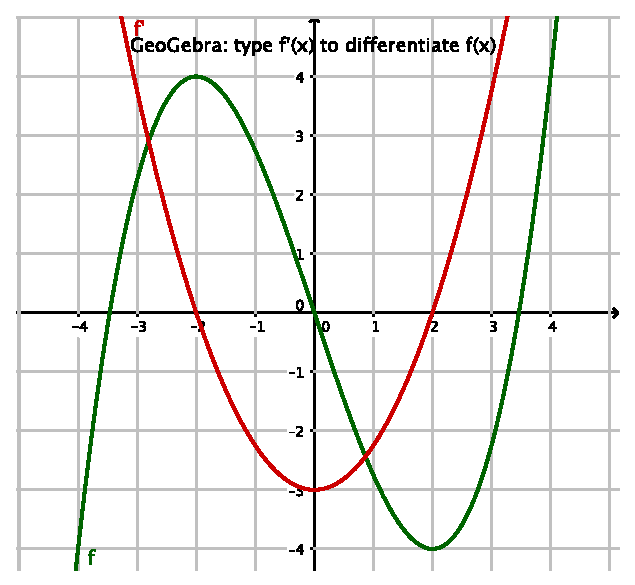
\includegraphics[height=0.7\textheight]{7-3_calc-ex-p208.eps}
  \end{figure}
}

\end{document}